% Template for PLoS
% Version 3.1 February 2015
%
% To compile to pdf, run:
% latex plos.template
% bibtex plos.template
% latex plos.template
% latex plos.template
% dvipdf plos.template
%
% % % % % % % % % % % % % % % % % % % % % %
%
% -- IMPORTANT NOTE
%
% This template contains comments intended 
% to minimize problems and delays during our production 
% process. Please follow the template instructions
% whenever possible.
%
% % % % % % % % % % % % % % % % % % % % % % % 
%
% Once your paper is accepted for publication, 
% PLEASE REMOVE ALL TRACKED CHANGES in this file and leave only
% the final text of your manuscript.
%
% There are no restrictions on package use within the LaTeX files except that 
% no packages listed in the template may be deleted.
%
% Please do not include colors or graphics in the text.
%
% Please do not create a heading level below \subsection. For 3rd level headings, use \paragraph{}.
%
% % % % % % % % % % % % % % % % % % % % % % %
%
% -- FIGURES AND TABLES
%
% Please include tables/figure captions directly after the paragraph where they are first cited in the text.
%
% DO NOT INCLUDE GRAPHICS IN YOUR MANUSCRIPT
% - Figures should be uploaded separately from your manuscript file. 
% - Figures generated using LaTeX should be extracted and removed from the PDF before submission. 
% - Figures containing multiple panels/subfigures must be combined into one image file before submission.
% For figure citations, please use "Fig." instead of "Figure".
% See http://www.plosone.org/static/figureGuidelines for PLOS figure guidelines.
%
% Tables should be cell-based and may not contain:
% - tabs/spacing/line breaks within cells to alter layout or alignment
% - vertically-merged cells (no tabular environments within tabular environments, do not use \multirow)
% - colors, shading, or graphic objects
% See http://www.plosone.org/static/figureGuidelines#tables for table guidelines.
%
% For tables that exceed the width of the text column, use the adjustwidth environment as illustrated in the example table in text below.
%
% % % % % % % % % % % % % % % % % % % % % % % %
%
% -- EQUATIONS, MATH SYMBOLS, SUBSCRIPTS, AND SUPERSCRIPTS
%
% IMPORTANT
% Below are a few tips to help format your equations and other special characters according to our specifications. For more tips to help reduce the possibility of formatting errors during conversion, please see our LaTeX guidelines at http://www.plosone.org/static/latexGuidelines
%
% Please be sure to include all portions of an equation in the math environment.
%
% Do not include text that is not math in the math environment. For example, CO2 will be CO\textsubscript{2}.
%
% Please add line breaks to long display equations when possible in order to fit size of the column. 
%
% For inline equations, please do not include punctuation (commas, etc) within the math environment unless this is part of the equation.
%
% % % % % % % % % % % % % % % % % % % % % % % % 
%
% Please contact latex@plos.org with any questions.
%
% % % % % % % % % % % % % % % % % % % % % % % %

\documentclass[10pt,letterpaper]{article}
\usepackage[top=0.85in,left=2.75in,footskip=0.75in]{geometry}

% TODO remove before submission
\usepackage{mathptmx}

% Use adjustwidth environment to exceed column width (see example table in text)
\usepackage{changepage}

% Use Unicode characters when possible
\usepackage[utf8]{inputenc}

% textcomp package and marvosym package for additional characters
\usepackage{textcomp,marvosym}

% fixltx2e package for \textsubscript
\usepackage{fixltx2e}

% amsmath and amssymb packages, useful for mathematical formulas and symbols
\usepackage{amsmath,amssymb}

\DeclareMathOperator*{\argmin}{arg\,min}

\DeclareMathOperator*{\argmax}{arg\,max}

% cite package, to clean up citations in the main text. Do not remove.
\usepackage{cite}

% Use nameref to cite supporting information files (see Supporting Information section for more info)
\usepackage{nameref,hyperref}

% line numbers
\usepackage[right]{lineno}

% ligatures disabled
\usepackage{microtype}
\DisableLigatures[f]{encoding = *, family = * }

% rotating package for sideways tables
\usepackage{rotating}

% Remove comment for double spacing
%\usepackage{setspace} 
%\doublespacing

% Text layout
\raggedright
\setlength{\parindent}{0.5cm}
\textwidth 5.25in 
\textheight 8.75in

% Bold the 'Figure #' in the caption and separate it from the title/caption with a period
% Captions will be left justified
\usepackage[aboveskip=1pt,labelfont=bf,labelsep=period,justification=raggedright,singlelinecheck=off]{caption}

% Use the PLoS provided BiBTeX style
\bibliographystyle{plos2015}

% Remove brackets from numbering in List of References
\makeatletter
\renewcommand{\@biblabel}[1]{\quad#1.}
\makeatother

% Leave date blank
\date{}

% Header and Footer with logo
\usepackage{lastpage,fancyhdr,graphicx}
\usepackage{epstopdf}
\pagestyle{myheadings}
\pagestyle{fancy}
\fancyhf{}
\lhead{\includegraphics[width=2.0in]{PLOS-submission.eps}}
\rfoot{\thepage/\pageref{LastPage}}
\renewcommand{\footrule}{\hrule height 2pt \vspace{2mm}}
\fancyheadoffset[L]{2.25in}
\fancyfootoffset[L]{2.25in}
\lfoot{\sf PLOS}

\usepackage{subcaption}

%% Include all macros below

\newcommand{\lorem}{{\bf LOREM}}
\newcommand{\ipsum}{{\bf IPSUM}}

%%%%%%%%%%%%%%%%%%%%%%%%%% REMOVE BEFORE SUBMISSION %%%%%%%%%%%%%%%%%%
\usepackage[colorinlistoftodos]{todonotes}




%% END MACROS SECTION


\begin{document}
\vspace*{0.35in}

% Title must be 250 characters or less.
% Please capitalize all terms in the title except conjunctions, prepositions, and articles.
\begin{flushleft}
%{\Large
%\textbf\newline{Can We Identify Transmission Bias in the Archaeological Record?  An Investigation of Equifinality Using Classifier Methods}
%}
{\Large
\textbf\newline{We Cannot Easily Identify Biased Cultural Transmission in the Archaeological Record}
}
\newline
% Insert author names, affiliations and corresponding author email (do not include titles, positions, or degrees).
\\
Mark E. Madsen\textsuperscript{1,*}


\bf{1} Department of Anthropology, Box 353100, University of Washington, Seattle, WA 98195-3100, USA
\\
\bigskip

% Insert additional author notes using the symbols described below. Insert symbol callouts after author names as necessary.
% 
% Remove or comment out the author notes below if they aren't used.



% Use the asterisk to denote corresponding authorship and provide email address in note below.
* mark@madsenlab.org

\end{flushleft}
% Please keep the abstract below 300 words
\section*{Abstract}
Lorem ipsum dolor sit amet, consectetur adipiscing elit. Curabitur eget porta erat. Morbi consectetur est vel gravida pretium. Suspendisse ut dui eu ante cursus gravida non sed sem. Nullam sapien tellus, commodo id velit id, eleifend volutpat quam. Phasellus mauris velit, dapibus finibus elementum vel, pulvinar non tellus. Nunc pellentesque pretium diam, quis maximus dolor faucibus id. Nunc convallis sodales ante, ut ullamcorper est egestas vitae. Nam sit amet enim ultrices, ultrices elit pulvinar, volutpat risus.


\linenumbers

\section{Introduction}\label{introduction}

A major use of cultural transmission models in archaeology is inference
regarding the mode of transmission operative within past populations.
Identifying cognitive biases is central, for example, to several
hypotheses for the origin of cumulative cultural transmission and
complex culture \cite{BR1985, CF1981, Henrich:1998ek, Wakano:2007gq}.
In more recent archaeological contexts, the identification of
frequency-biased social learning has been used to support
inferences concerning sociopolitical structure 
in past societies \cite{kohler2004}.  Simulation and mathematical
studies have yielded many insights into the empirical patterns we can expect from different transmission models
\cite{Bentley2003, bentley2007regular, bentley2004random, Evans:2011vm, Mesoudi2009},
although much of this knowledge is derived from very simplified
population models.  In particular, theoretical analyses of transmission models  have ignored until recently the effect of data collection methods and coarse-grained observations on the patterns we should expect in archaeological data.  As a result, we simply do not know whether the mode of transmission can be reliably inferred from samples of the archaeological record, if it is possible at some time scales but not others, or how we might tailor data collection strategies to maximize the accuracy of such inferences.


We do know that the coarse graining of observable variables that occurs given time averaging reduces our ability to distinguish between
unbiased and biased transmission models
\cite{Madsen2012TA, Porcic2014Exploring-the-E, Premo:2014jv}, that non stationary
population sizes reduce our ability to infer transmission modes \cite{Rorabaugh:2014fl}, and that
diachronic statistics and non equilibrium models are better than
synchronic measures and equilibrium models 
\cite{kandler2013non, wilderkandler2015}.  The effect of these factors is such that when deposits are highly time averaged, equifinality occurs, with different models yielding the same empirical distributions despite describing different underlying processes \cite{von1949problems}. Equifinality between
theoretical models is a serious concern whenever we study complex
systems, and has been discussed in geomorphology, hydrology,
climatology, and within archaeology itself
\cite{Aronica:1998dm, Beven:2006js, Bonham:2009bi, Cicchetti:1996gp, 
Culling:1987kx, Marean:1992hg, Rogers:2000bq, Savenije:2001fe}.
If models which represent different modes of cultural transmission
cannot be distinguished when we include aggregation, heterogeneity, or sampling in our models,
then there may be questions concerning past cultural transmission that
we cannot answer.  As a result, there may be classes of models which are useful for contemporary or historical 
research, but not for the coarse grained scales of observation that archaeologists often confront.

Existing theoretical studies have almost exclusively focused upon distinguishing
models based on the ability of a single statistic or variable to
distinguish the distribution of outcomes from different social learning
modes. Scores from the power law exponent
in a log-log plot of trait frequencies have received the most attention along with more recent application of neutrality tests \cite{Bentley2003, bentley2004random, Mesoudi2009, slatkin1994exact, slatkin1996correction}.   
More recently, Kandler's work has demonstrated that diachronic measures such
as trait survival time, or the length of time the most common trait
stays ranked the most common, can be robust predictors of different
classes of transmission models
\cite{kandler2013non, wilderkandler2015}. 
But there is little reason to suspect that single statistics will be adequate in most cases to cleanly separate and identify different transmission models, given the strong convergence in distribution that characterize diffusion processes.  Instead, we should expect that statistical models employing multiple predictors would be the best discrimination tools, if any exist for a set of transmission models.  In this paper, I employ
a robust machine learning classifier algorithm and multiple ways of measuring
trait richness, diversity, and survival times to test whether
equifinalities exist between various combinations of unbiased and biased
transmission rules when measurements come from realistic data collection
scenarios.\footnote{Throughout this paper, I used ``classification'' in the statistical and machine-learning sense of a statistical model whose dependent variable is a binary or discrete value, such that the model predicts which value a data point takes from a labeled set.  Archaeologists will be used to using the term in the sense of systematics and taxonomy, which is not the intent here.}

The results indicate that while neutral and biased transmission models
can be distinguished very accurately given measurements from entire
populations taken when no temporal aggregation occurs, the introduction of
sampling and the interaction between sampling and time averaging
 markedly degrades our ability to distinguish these transmission
rules. Furthermore, the degradation is not symmetric. With sampled, time
averaged data, we are extremely likely to conclude that samples
represent biased transmission, even when this is not the case. Other
mixtures of conformist and anti-conformist transmission rules are even
less distinguishable given time averaging and limited samples.  As a result, I conclude that it may be difficult or impossible to infer the details of cognitively biased transmission rules from frequency data alone, when we lack data from an entire population and when only coarse grained, aggregated data are available.

\section{Analysis}\label{analysis}

\subsection{Reducible and Irreducible Equifinality Among Transmission
Models}\label{measuring-equifinality-among-transmission-models}

Equifinality among cultural transmission models can arise from several sources. First, equifinality may occur because of our measurement and analysis
procedures. There is growing evidence, for example, that assemblage
duration affects our ability to distinguish biased from neutral
transmission across a variety of statistical predictors
\cite{Madsen2012TA, Porcic2014Exploring-the-E, Premo:2014jv}. Equifinality among transmission models is thus possibly reducible by collecting finer-grained samples during fieldwork, if deposits are well stratified.  However, in situations where the depositional environment actively creates temporal aggregation (e.g., in the plowzone, or in deflated aeolian contexts), there may be little that an investigator can do to improve the temporal resolution of data collection.  And when we employ published data sets, obviously we cannot easily subdivide the data into assemblages finer than the original investigation supported.  When studying living populations, of course, equifinalities may be addressed by converting a purely observational study to a controlled experiment in some cases \cite{kempe2014experimental, mesoudi2014experimental, schillinger2014copying},
but of course this is not an option in archaeological contexts.

Second, equifinality is partially determined by the predictors or variables we use in trying to separate the behavior of models.  Fig. \ref{fig1} shows an artificial example with two distributions, measured on two variables.  The marginal distribution of each variable demonstrates how models might be distinguishable given one variable (Y axis) but not another (X axis).  In the published literature on transmission modes, single variables are usually examined, but we gain huge power by considering statistical models with multiple variables.  


\begin{figure}
	\caption{Simple example of the effect of variable choice in distinguishing models.  The variable on the X axis displays quite a bit of overlap between models, while the variable on the Y axis distinguishes the models with fairly high accuracy.}
	\label{fig1}
\end{figure}

Not all equifinalities may be reducible.  The statistical distributions generated by diffusion processes can be highly convergent among related models, and almost all cultural transmission models are, at base, diffusion processes. This type of equifinality is \textbf{irreducible}, and is not solved by changing how we perform the analysis or by changing data collection. Irreducibly equifinal
models form an \textbf{equivalence class} of models that we cannot
distinguish given our data. Instead, all we can say is that our data
could have been generated by any of the models in the equivalence class.  
If the equivalence classes of equifinal models are coarse enough (at worst, if they 
form a single group), then we cannot meet our original inferential goals at all. 

In some cases, irreducible equifinalities can become reducible given advances in measurement technologies that open up new sets of predictor variables.  After his seminal works of the 1970's on drift and the infinite-alleles neutral model, Warren Ewens stopped working on neutrality tests because tests using allele count data lack statistical power.  Ewens moved to studying the population genetics of human diseases instead \cite{plutinski2004}, recognizing that further progress would require sequence data unavailable at the time.  This judgment proved accurate:  a new suite of neutrality tests did arise starting the late 1980's and 1990's when sequence data became widely available \cite{fu1993statistical,tajima1989statistical}.     


\subsection{Equifinality As Classification Error}
\label{sec:equifinality-classification-error}

Since our evolutionary models of cultural transmission are stochastic, and generate a variety of outcomes for the same parameter values, I take a statistical approach to examining equifinality of transmission models in archaeological data.  Transmission modes are separable and thus identifiable in archaeological data if the distribution of model outcomes are non-overlapping, when measured in a space created by a set of predictor variables.  With stochastic models like the ones currently used by archaeologists, the most efficient method of studying the outcome distribution is to simulate values from the model, and examine our ability to correctly predict which model generated each data point, given a function of the predictor variables.  

This general approach can be visualized as in Fig.
\ref{fig2}. Here, three pairs of probability models
are represented by 500 measurements each of two continuous predictors variables (e.g., a diversity index).
In the left panel, the pair of models do not overlap in their outcomes.
Given a data point, we can assign it to Model 1 or Model 2 with
virtually no error, and thus we would consider models 1 and 2 to be
distinct and not equifinal at all. The situation in the middle and right
panels of Figure \ref{fig1} is different. There is
some overlap in the middle panel, and very strong overlap in the right
panel. In the right hand panel, in fact, there is enough overlap that on
average, our ability to assign a randomly chosen data point to the
correct model is no better than chance. Intuitively, we would say that
there is some equifinality in the middle panel, and that the two models
were strongly equifinal in the right hand panel.

\begin{figure}[h]
\caption{Simple example of model outcomes with different degrees of distinguishability: (A) simulated data point from two fully separate models, (B) two models with a limited overlap region, (C) and two models whose outcomes are highly overlapping.}
\label{fig2}
\end{figure}


We can formalize the analysis of overlap between models as a problem of
``classification'' or ``pattern recognition'' in the sense of
statistical or machine learning \cite{hastie2009elements}. Given a set
of models \(\mathcal{M}_1 \ldots \mathcal{M}_n\), we can measure
equifinality as the minimum possible error achievable in correctly
assigning simulated data points to the models which generated them,
given measurement of a set of predictor variables. In general, the
classification problem asks which model has the highest probability for
a given data point, given the conditional density of the data and
models. This sounds exactly like Bayes' theorem, and in fact we can
write the classification problem as follows, where
\(Y \in 1, \ldots, K\) refers to each of \(k\) models, and
\(X_1, \ldots, X_p\) refer to \(p\) different predictor variables.

\begin{equation}
\mathbb{P}(Y | X_1, \ldots, X_p) = \frac{\mathbb{P}(Y_i) \mathbb{P}(X_1, \ldots, X_p | Y)}{\mathbb{P}(X_1, \ldots, X_p)}
\label{eq:bayes-rule-classification}
\end{equation}

\(\mathbb{P}(Y)\) plays the role of the prior distribution, and is the
prevalence of each model in the population. This is a constant in
situations where we are simulating values from each model to test for
equifinality. The data points in a classification problem are given, and
thus the denominator is a constant. The most probable class for a given
data point is just the mode of the likelihood function, which is given
by:

\begin{equation}
Y_{pred} = \argmax_y \mathbb{P}(X_1, \ldots, X_p | Y)
\label{eq:map-class-bayes}
\end{equation}

This is the \emph{Bayes classifier} for a controlled simulation
experiment, and its error rate in separating data points by model is
called the \emph{Bayes error}. This is the lowest possible error in
separating the models given the data
\cite{devijver1982pattern, fukunaga1990introduction, hastie2009elements}.
The Bayes error is zero when we can correctly identify each data point
as to its model of origin (as in the left panel of Fig. \ref{fig2}, and rises as two models overlap in the
measurement space. With sufficient overlap, the Bayes error could
approach 0.5, which represents a prediction rule which is no better than
chance.\footnote{Predictors can achieve even worse error levels, performing more poorly than coin-flipping, but in the current study we will not encounter such rates.}

Unfortunately, we can almost never directly calculate the Bayes error
rate for a prediction or classification rule, because we rarely have an
expression for the likelihood function of our transmission models in the
spaced formed by the predictor variables. Bayes error can be directly calculated, in fact, only for
a small number of cases, such as Gaussian distributions with a shared
covariance
matrix.\footnote{There is a large literature, especially in pattern recognition and language classification, on approximating upper bounds for the Bayes error of a classifier, because it is highly useful to know when you cannot improve a recognition system or classifier any further \cite{Antos:1999dn, Dobbin:2009du, McLachlan:1975eo}.  Most such upper bounds are based upon parametric models, and use estimates of a distance metric between the classes being distinguished (typically, the Mahalanobis or Bhattacharyya distance) \cite{devijver1982pattern}.  Such bounds are difficult to justify in situations where we have complex social learning models, whose probability density functions in the space of measured variables are typically unknown and are unlikely to be Gaussian.  Non parametric bounds are possible, using nearest-neighbor methods \cite{Loizou:1987bi}, but in most cases the values obtained are not very tight and the performance of boosting and bagged classifiers easily surpasses such methods.}
Despite the fact that we can rarely calculate the Bayes error rate, it
is useful as an operational definition for equifinality, since it
measures our uncertainty about model choice given a set of measurable
variables. In practice, we approximate the Bayes error by employing
algorithms which are known to have near-optimal performance in
classification problems. In particular, boosting, bagging, and ensemble
approaches that combine many classifier rules are attractive since each
achieves some of the best generalization error in prediction tests
\cite{hastie2009elements}, and thus come closest to estimating the
Bayes rate \cite{tumer2003bayes}.  


\subsection{Study Design}\label{model-comparisons}

To examine whether a classifier approach with multiple predictor variables, allows us to identify modes of cultural transmission in archaeological data, this study simulates four different transmission models, and compares our ability to correctly identify data points in a series of three pairwise comparisons between models.  The transmission models include:

\begin{enumerate}
\def\labelenumi{\arabic{enumi}.}
\itemsep1pt\parskip0pt\parsep0pt
\item
  Unbiased or neutral cultural transmission
\item
  Mixture of equal numbers of conformists and anti-conformists.
\item
  A mixture dominated by conformists, but with 30\% anti-conformists.
\item
  A mixture dominated by anti-conformists, but with 30\%
  anti-conformists.
\end{enumerate}

Unlike previous theoretical studies of cultural transmission models in anthropology, I study mixtures of transmission modes since real populations are typically heterogeneous.  We might also expect that certain mixtures of biased transmission might be statistically difficult to distinguish.  For example, an equal mixture of conformist and anti-conformists might cancel out each other's biases, and thus be difficult to separate from a population of unbiased individuals who copy one another randomly. This study focuses, therefore, on three pairwise comparisons drawing upon the four models just described:

\begin{table}[h]
\begin{tabular}{lll}
\hline
Comparison & Model \#1 & Model \#2 \\ 
\hline
Neutral vs. Biased & Unbiased transmission & All 3 biased models \\
Neutral vs. Balanced Bias & Unbiased transmission & Equal number of pro/anti conformists \\
Pro/Anti Conformism & Conformist dominated & Anti-conformist dominated  \\
\hline
\end{tabular}

\caption{Model comparisons tested in this study for equifinality.}
\label{tab:comparisons}
\end{table}

In addition to comparing different mixtures of transmission modes, we want to determine the extent to which equifinality (if it occurs) is affected by the conditions of data collection.  Thus, for each set of simulations from a model, a standard set of predictor variables is measured for a variety of levels of sampling from the simulated population, and temporal aggregation of copying events.  The extent to which equifinality occurs for some data collection regimes, but not others, is an indication that the equifinality is potentially reducible by augmenting sample size or obtaining finer-grained, less time averaged samples. To the extent that equifinality exists regardless of data collection strategy, the study might identify irreducible equifinalities between specific model pairs.  

The general process followed throughout the study is:

\begin{itemize}
\itemsep1pt\parskip0pt\parsep0pt
\item
  Simulate a large number of samples from each cultural transmission
  model, given a range of parameters.
\item
  Measure a set of archaeologically relevant variables (e.g., richness,
  diversity) on each sample
\item
  Perform each variable measurement across different data collection
  regimes (e.g., duration of accumulation, sample size)
\item
  Train a predictive classifier model for each data collection regime,
  to predict the model of origin given the measured variables
\item
  Assess the classifier error rate using additional samples simulated
  from each transmission model
\end{itemize}


%Given simulated output from each of the four models, I performed three
%model comparisons in order to detect equifinality (Table
%\ref{tab:comparisons}). First, I compare unbiased transmission to all
%three of the biased models, to determine whether (and under what data
%collection conditions), we can simply distinguish bias in general from
%neutral or unbiased copying. Second, I compare whether unbiased
%transmission can be distinguished from a ``balanced'' mixture of
%conformist and anti-conformist copying, where each bias rule is held by
%50\% of the population. In principle, the biases may cancel their
%effects and yield population-level results which look unbiased. Third, I
%compare whether a population dominated by conformists can be
%distinguished from a population dominated by anti-conformists. I
%anticipate that the order in which these comparisons are described may
%correspond to the difficulty of distinguishing these models in
%population-level data.

\subsection{Methods}\label{methods}

\subsubsection{Simulated Samples of Cultural Transmission
Models}\label{simulated-samples-of-cultural-transmission-models}

The outcomes of all four transmission models are derived by simulating the
dynamics of the model in an agent-based framework that allows each agent to be assigned a different transmission rule.  All simulations employ
the Moran dynamics, where one individual engages in a copying event at
each elemental step
\cite{moran1962statistical, moran1958random, aoki2011rates}.
Innovations are modeled using the ``infinite alleles'' approximation,
where every innovation is new to the population \cite{Ewens2004}.
Simulations were performed using the CTMixtures software package,
available as open source
software.\footnote{\url{https://github.com/mmadsen/ctmixtures}} The
parameters for all simulation runs are given in Table
\ref{tab:parameters}. Where there is a range given (e.g., innovation
rate), the parameter is treated as a prior distribution and each
simulation run is assigned a uniform random value from the range. This
ensures good coverage of the parameter space given 25,000 replicates for
each of the 4
models.\footnote{The use of a good prior distribution for parameter ranges also results in simulation data that are usable for later data fitting by approximate Bayesian inference \cite{Beaumont:2010ur, Crema:2014ef, Csillery:2010jd, marin2012}.}

\begin{table}[h]
\begin{tabular}{lc}
\hline
Parameter & Value or Interval \\ 
\hline
Innovation rate (in $\theta$ scaled units)  & $[0.1, 5.0]$   \\
Probability of conformism & $[0.05, 0.25]$ \\
Probability of anti-conformism & $[0.05, 0.25]$ \\
Sample fractions & 0.1 and 0.2 \\
Time averaging intervals (units of 100 individuals) & 10, 20, 50, 100 \\
Population size & 100 \\
Number of trait dimensions (loci) & 4 \\
Initial traits per dimension & 10 \\
\hline
\end{tabular}

\caption{Parameters for simulation runs across the four models studied.  Intervals are treated as prior distributions, and each simulation run is assigned values derived from a uniform random sample on the interval indicated.  Lists of values are all applied to every simulation run (e.g., there is both a 10\% and a 20\% sample from each simulation run.  Single values are applied to every simulation run, and represent a point prior.)}
\label{tab:parameters}
\end{table}

Simulated populations are 100 individuals in size, because most
archaeological studies of cultural transmission have focused upon
situations where population sizes are assumed to be small. 
Each simulated individual carries 4 different
traits at any time, which are treated as separate loci or dimensions.  Trait frequencies are tracked on a per-locus basis, and combinations of loci are tracked in order to simulate archaeological ``types'' or classes which include multiple dimensions of variation.

Regardless of transmission model, social learning involves no interaction effects between loci in this study. The
population is seeded with 10 randomly chosen traits at each locus as a
starting configuration. The evolution of each simulated population proceeds
for 4 million elemental steps, which is equivalent to about 40,000
copying events on average per individual. This value was chosen by
performing simulations at 1 million time step intervals and verifying
that the distribution of a key statistic (the number of traits per Loci)
had stabilized. This occurred in most cases between 2 and 3 million
steps, and in all cases between 3 and 4 million, so the last value
was chosen.\footnote{The analysis underpinning this decision is available in the Github repository at \url{https://github.com/mmadsen/experiment-ctmixtures/analysis/verification}.}
At the end of 4 million simulation steps, a suite of variables are
measured from each of the 25,000 replicates and stored for analysis.

\subsubsection{Variable Selection}\label{variable-selection}

Since most previous work on identifying transmission mode from archaeological data employ single diagnostic variables, and begin to display equifinality under realistic data collection conditions, it is reasonable to examine whether using multiple variables will yield more discriminatory power in the same contexts.  By representing the outcomes of transmission models in a higher dimensional space, it should be easier to find a decision boundary (``separating hyperplane'') that correctly predicts the model which generated each data point, if such a boundary exists.  

\begin{table}[ht]
\begin{tabular}{lll}
\hline
Variable                                    & Model Variable \\ 
\hline
Cross-Tabulated Class Richness  (Class)         &  num\_trait\_configurations      \\
Slatkin Exact (Class)           & configuration\_slatkin       \\
Shannon Entropy (Class)  &  config\_entropy \\
IQV Diversity (Class)  & config\_iqv \\
Neiman $T_f$ (Class) & config\_neiman\_tf \\
Slatkin Exact (Max for Locus)                    & slatkin\_locus\_max       \\
Slatkin Exact (Min for Locus)                     & slatkin\_locus\_min      \\
Slatkin Exact (Mean for Locus)                   & slatkin\_locus\_mean       \\
Shannon Entropy of Trait Frequencies (Min)      & entropy\_locus\_max       \\
Shannon Entropy of Trait Frequencies (Max)       & entropy\_locus\_min      \\
Shannon Entropy of Trait Frequencies (Mean)      & entropy\_locus\_mean      \\
IQV Diversity Index (Min)     & iqv\_locus\_max \\
IQV Diversity Index (Max)     & iqv\_locus\_min \\
IQV Diversity Index (Mean)    & iqv\_locus\_mean \\
Trait Richness (Min)   & richness\_locus\_max \\ 
Trait Richness (Max)   & richness\_locus\_min \\
Trait Richness (Mean)    & richness\_locus\_mean \\
Kandler-Shennan Trait Survival (Min)   & kandler\_locus\_max \\
Kandler-Shennan Trait Survival (Max)   & kandler\_locus\_min \\
Kandler-Shennan Trait Survival (Mean)   & kandler\_locus\_mean \\
Neiman $T_f$ (Min)   & neiman\_tf\_locus\_max \\
Neiman $T_f$ (Max)   & neiman\_tf\_locus\_min \\
Neiman $T_f$ (Mean)   & neiman\_tf\_locus\_mean \\
\hline

\end{tabular}

\caption{Variables measured from each transmission model simulation sample.  The parenthetical expression records whether the variable was calculated for cross-tabulations of all 4 loci (Class) or represent the order statistics from individual loci (Min/Mean/Max).  The right column records the variable name used within R statistical models, for examining the relative importance of each variable in classifying observations.}
\label{tab:variables}
\end{table}

The predictor variables chosen in this study focus upon measures of richness and
diversity, trait survival over time \cite{kandler2013non}, and the
Slatkin neutrality test \cite{slatkin1996correction, slatkin1994exact}.
Each has been employed in the archaeological literature on identifying
cultural transmission modes, or is a variant on such measures (e.g., IQV
is a normalized version of Shannon entropy), and crucially, all are measurable in standard archaeological contexts using type frequency data.  This additionally makes most of the variables applicable to the re-analysis of already published data, which is an important usage scenario in archaeological research.   

For the locus-centric variables, each statistic was applied to each
locus separately, and the mean, minimum, and maximum of the values
obtained for each locus were recorded. I collect order statistics
in addition to the mean value, since it is possible that minima and
maxima might be a better discriminator between models than averages. In
addition to the variables calculated upon each of the 4 loci, the traits
at each locus were combined into a cross-tabulation of "classes" which simulates the
process of archaeological classification. Each class represents a
different combination of traits from the 4 loci, and very roughly
simulates observing cultural variation through the lens of a standard
paradigmatic classification \cite{Dunnell1971}. The same variables are
then measured as a function of the class counts.\footnote{The sole exception is the Kandler-Shennan survival time, which is not measured here for the cross-tabulated classes.  Understanding the quantitative behavior of this measure for multidimensional classes of traits is an important open research question, however.} This allows us to
understand whether transmission models are better distinguished on a
per-locus (dimension) basis or by operating on more complex classes that
combine several traits together. The full list of measured variables is
given in Table \ref{tab:variables}.

As a final note on variable selection, in an exploratory analysis for this
project, I tried to include the power law exponent from a log-log
transformation of trait frequency, given the important work by Bentley
\cite{bentley2004random} and Mesoudi and Lycett
\cite{Mesoudi2009}. It is not clear, however, that previous uses
of this variable have been comparable to measurements we can make on
archaeological assemblages. As an example, Mesoudi and Lycett
\cite{Mesoudi2009} use the cumulative number of adoptions of each
trait over the entire time span of the simulation as the ``frequency''
used to calculate power law
exponents.\footnote{I confirmed this by inspection of the source code for their simulation model, which was provided by Alex Mesoudi.}
Given the measurement strategies described in Table
\ref{tab:measurement-strategies}, the number of traits present at any
given time is often small, and their prevalence in a small population
makes it difficult to fit a power law to the data. Despite its
importance in archaeological discussions of neutral versus biased
transmission, I have omitted power law exponents from the published
analysis, pending investigation of the proper method for calculating
them in situations with small \(N\) and small numbers of trait
categories.

\subsubsection{Data Collection Treatments}\label{data-collection-treatments}

At the end of each simulation run, after the model has reached a quasi-stable equilibrium (measured as stability in per-locus trait richness), a series of samples are taken from the evolving population.  These samples are taken in ways that correspond to various real-world data collection strategies.  First, a census of the entire population is taken.  This functions as a baseline for the ``most complete'' information we can use to identify transmission modes, and there are also conditions during observational studies or in laboratory experiments where census is possible.  In archaeological studies, anything approximating a census is usually impossible, although Jonathan Scholnick's study of New England gravestones and their makers may approximate this quality of data collection \cite{scholnick2012spatial}.  Second, the simulated population is sampled, at the 10\% and 20\% levels.  Sampled data is ubiquitous in archaeological research, and although the issues involved in mapping artifact samples to their meaning for the underlying population of social learners is complex and unresolved, it is useful to determine whether the overall sample fraction has a measurable effect upon model equifinality.  

Archaeological data are rarely synchronic or ``point in time'' samples of the results of human activity, and are typically aggregated over an appreciable duration of time through both data recovery conventions and formation processes \cite{grayson1998,lyman2003influence,Madsen2012TA,Porcic2014Exploring-the-E,Premo:2014jv}.  Thus, the sampled data employed in this study is also temporally aggregated over a number of time steps, and the aggregate trait counts and then used to determine the frequencies of cultural traits over the entire interval.  The population census has no temporal aggregation, and thus does represent a synchronic census.  

Time averaging is implemented according to the schematic in Fig. \ref{fig3}.  At the end of the simulation run, sampling begins at a time index calculated to allow time averaged samples to be taken twice, with a gap of 50 ``generations'' to allow the calculation of the Kandler-Shennan trait survival statistic (although unlike their original study, the values at the start and end times are inherently time averaged in this study, which would be the base in any real archaeological context) \cite{kandler2013non}.\footnote{The effect of time averaging on the start and end values used to calculate the Kandler-Shennan trait survival is not directly studied in this paper, but is a necessary component of using their method to study archaeological assemblages, I believe.}  

\begin{figure}[h]
	\caption{Schematic of how sampling is implemented in this study.  Time runs from the start of the simulation run at the top, to the end at the bottom.  The interval of time over which we calculate the Kandler-Shennan trait survival is given as a simulation parameter, and represents the gap in the middle of the diagram.  Before and after that gap are windows of successive duration, representing aggregation over 10, 25, 50, and 100 ``generations'' of the simulation.}
	\label{fig3}
\end{figure}


\begin{table}[ht]
    \begin{tabular}{lll}
        \hline
        Sampling Strategy & Time Averaging Duration \\ 
        \hline
        Population Census & 0 \\
        10\% Sample & 10 \\
        10\% Sample & 25  \\
        10\% Sample & 50 \\
        10\% Sample & 100 \\
        20\% Sample & 10  \\
        20\% Sample & 25 \\
        20\% Sample & 50 \\
        20\% Sample & 100 \\
        \hline
    \end{tabular}
    \caption{Data collection strategies, applied to every simulation run.  Time averaging duration is given in units of "generations," which are units of 100 time steps (given the population size).  100 generations thus represents 10,000 elemental time steps in the Moran simulation dynamics.}
    \label{tab:measurement-strategies}
\end{table}

The data collection strategies employed in this study are given in Table \ref{tab:measurement-strategies}.  Applied to all 23 variables, the study yielded approximately 900,000 samples from the four transmission models.\footnote{All data and analyses for this study are available as part of a Github repository, although large data files are kept on Amazon S3 for long-term storage.  See \url{https://github.com/mmadsen/experiment-ctmixtures} for details.  The published analysis described here is the ``equifinality-4'' data set.}  This raw data was then formed into the three pairwise comparisons shown in Table \ref{tab:comparisons} for equifinality analysis with a classifier model.

\subsubsection{Classifier Selection and
Training}\label{classifier-selection-and-training}

Classifier algorithms are supervising learning models from statistics
and machine learning that predict a categorical response from a mixture
of discrete or continuous variables \cite{hastie2009elements}. The most
familiar classifiers in archaeological practice are logistic regression
and discriminant function analysis, but neither is competitive with
contemporary ``ensemble'' methods which combine many classifier rules
into a single prediction. In such models, combining predictors can both
reduce the variance of prediction (e.g., bagging added to traditional
classifiers and random forests), and
reduce bias.  Some classifiers, like boosted trees, can do both.

Since the Bayes error rate of comparing two complex transmission models is not something we can calculate or even estimate, we must approximate it using the best performing classifier model available.  A very general result in statistical
decision theory (called, appropriately, the ``No Free Lunch'' theorems)
guarantee that there is no single prediction model that can achieve the
best result with every data set and problem
\cite{wolpert2002supervised, wolpert1997no}. Thus, I took a compromise approach, selecting several algorithms that are known to have excellent performance across a range of data sets, and then performing a pilot study using the four transmission models previously described.  A recent study
compared 179 classifier algorithms on 121 different data sets
(representing the entire UC Irvine Machine Learning Database), and found
that random forests \cite{breiman2001random}, support vector machines,
and gradient boosted classifiers performed the best
\cite{hastie2009elements}. Additionally, some ensemble methods (random
forests and gradient boosted classifiers) provide information on
variable importance as an integral part of the algorithm.  Since understanding which of our 23 variables are useful for separating transmission models is an important aspect of this study, I evaluated random forests against gradient boosted classification trees using small simulated samples from each transmission model.\footnote{The data for this initial comparison are available in the \url{https://github.com/mmadsen/experiment-ctmixtures} repository under the experiment name ``equifinality-2''.}
Gradient boosted models outperformed random forests on these simulated
data, are comparable in computational costs, and are used for all
further results in this paper.

Gradient boosted classification operates by repeatedly fitting a set of
decision trees to the data \cite{AlexeyNatekin:2013ew,hastie2009elements}. In each round, decision trees are fit to the training data, and individual data points scored as errors or successful predictions.  Subsequent trees are fitted by modifying the trees in the direction that minimizes the residual error.  This is equivalent to finding the gradient of the loss function in the space of possible classifier functions, hence the name of the method.  The impact of each gradient step is smoothed by including a ``shrinkage'' factor.  Finally, the gradient steps are ``boosted'' to weight data points by the success in prediction, such that data points that are frequently misclassified become targeted by the algorithm until they can be correctly predicted \cite{freund1995boosting, freund1999short, schapire2012boosting}.  After a specified number of iterations, the class or label membership of each data point is obtained by having each gradient step classifier tree ``vote'' for class membership, and the final answer is the majority vote.  This class of models can also be visualized as repeated refitting of residuals until error is minimized \cite{friedman2001greedy}.  This combination of boosting and iterative function search is very powerful, and gradient boosted models regularly achieve top accuracy in benchmark studies.

In this study, I employ the R package (\textbf{gbm}) for gradient
boosted classification \cite{ridgeway1999state}, with the binomial deviance \(\textrm{log}(1 + \textrm{exp}(-2y\hat{y}))\) as our loss function, where \(y\) is the true
model for a data point, and \(\hat{y}\) is the classifier model's
prediction.  Binomial deviance approximates the ``zero-one'' loss function with one which is differentiable, which is needed for a gradient descent method.  The tuning parameters for this study (number of boosting iterations, depth of classification trees) were selected using 5 rounds of repeated 10-fold cross-validation on the training data \cite{Kim:2009im, kuhn2013applied}.

The full data set is  split into two chunks. 80\% of the data are
used to train the classifier model, and 20\% are held back to provide an
unbiased evaluation of classifier performance.  For each comparison of models
reported here, the training data are thus fitted 50 times across
different values of the tuning parameters (number of boosting
iterations, and depth of decision trees), and the best performing
parameters chosen from the repeated cross-validation sets. The final model is then constructed using the entire
training set and the optimal parameter values. All classifier tuning,
final model fitting, and test error evaluation was performed using Max
Kuhn's superb \textbf{caret} package for R
\cite{kuhn2008building, kuhn2013applied}.

\begin{table}[ht]
\begin{tabular}{c|cc}
 & Actual Model: & \\
 Predicted &  Model 1 & Model  2 \\
  \hline
 Model  1 & \textbf{9000} & 2500 \\
   Model  2 & 1000 & \textbf{7500} \\
\end{tabular}
    \caption{Example confusion matrix.  Columns correspond to the actual model for data points, rows correspond to predictions from a classification model.  Bold numbers on the diagonal correspond to correct predictions, the off diagonal elements correspond to classification errors.}
    \label{tab:confusion-matrix}
\end{table}


\subsubsection{Classification Error and Equifinality
Assessment}\label{classification-error-and-equifinality-assessment}




The basic data for assessing the quality of a classifier model is the
\emph{confusion matrix}, which compares classification successes and
errors for a data set.  A hypothetical example is given in Table
\ref{tab:confusion-matrix}.  The most basic measure of classification quality is the \emph{accuracy}, or the ratio
of correct predictions to the total number of data points.  In the confusion matrix, this is the ratio of the sum of diagonal elements to the sum of off-diagonal elements.  In the example given in Table \ref{tab:confusion-matrix}, the classifier is 82.5\% accurate. We often also use the misclassification rate, which is simply $1 - \textrm{accuracy}$.  


When the classes
being predicted are not balanced, and especially if there are a small
number of one class compared to another, a better statistic is Cohen's
``kappa'' \cite{kuhn2013applied}, which compares observed accuracy to
what one would expect purely from chance, given the marginal totals:

\begin{equation}
\kappa = \frac{O - E}{1 - E}
\label{eq:kappa}
\end{equation}

where \(O\) is the observed accuracy, and \(E\) is the expected accuracy
due to chance given the ratio of classes in the marginal totals of the
confusion matrix. Kappa ranges from \(-1\) to \(+1\), with \(0\)
indicating no agreement between predictions and the real class
memberships. High values indicate good agreement, while values below
\(0.5\) and especially less than \(0.2\) indicate very poor predictive
ability \cite{altman1991practical}. In the present context, a
classifier comparison (for example, biased versus neutral models with no
sampling or time averaging) that yield a high kappa value are strong
evidence that no equifinality exists between the two situations, since
the classifier is highly accurate. Low kappa values are evidence that
despite strong statistical methods and many variables to choose from, we
cannot distinguish between models, and thus the models may be equifinal.  

In studies where one outcome or class represents the presence of something (e.g., a positive test for a disease marker) and the other the absence, we may look at the individual cells of the confusion matrix rather than the bulk accuracy.  The ``false positive rate'' (FPR), for example, is the number of cases which are not members of the ``positive'' class, but which the classifier falsely identifies as such (in the example shown here, if Model 1 is the positive class, the cell in the upper right corner of the matrix is the FPR.  A number of other statistics build from FPR and the false negative rate to handle asymmetric experiments.  In the present study, we are interested simply in the misclassification rate, or bulk accuracy, of predicting the correct model.  Throughout these results, I use the misclassification rate and Cohen's kappa values exclusively.  

\section{Results}\label{results}

In the next three sections, I review the results of applying the gradient boosted classifier to the three pairwise comparisons described in Table \ref{tab:comparisons}.  

\subsection{Unbiased Versus Biased Cultural
Transmission}\label{unbiased-versus-biased-cultural-transmission}

In the first comparison, all data points generated by unbiased (neutral) cultural transmission form one class, and the data points generated by each of the 3 biased models.  As a reminder, the latter are:

\begin{enumerate}
\def\labelenumi{\arabic{enumi}.}
\itemsep1pt\parskip0pt\parsep0pt
\item
  Mixture of equal numbers of conformists and anti-conformists.
\item
  A mixture dominated by conformists, but with 30\% anti-conformists.
\item
  A mixture dominated by anti-conformists, but with 30\%
  anti-conformists.
\end{enumerate}

This comparison examines the question of whether multiple predictor variables give us the power to discriminate between unbiased and any mixture of biased transmission, across different data collection regimes.  For this comparison, classifier models were also developed for all of the predictor variables, and just for the per-locus variables, to determine the effect of using multidimensional classes that mimic archaeological classification, as opposed to simply examining single dimensions of variation (which has been the most common practice in archaeological studies to date).  

The results are summarized in Fig. \ref{fig4} as Cohen's kappa values across the different predictor variable sets and data collection regimes.  It is immediately apparent that multiple variables in our classifier model gives us great power in distinguishing biased from unbiased transmission, in the case where we have population census data which is not subject to temporal aggregation.  The use of multidimensional classes \emph{in addition} to per-locus variables offers a tiny increase in accuracy, but these two comparisons are otherwise equivalent and display no equifinality given 97\% accuracy in predicting biased versus unbiased transmission in the hold-out test set.  

\begin{figure}[h]
\caption{Cohen's kappa for correctly predicting whether simulated data points originate from unbiased copying or any of 3 other biased transmission models.  High values of kappa correspond to high accuracy in correctly distinguishing between transmission models, while values well below 0.5 indicate great difficult and low classifier accuracy.  Each line in the dotchart represents a different data collection treatment, and overall the results indicate that significant equifinality exists except when time averaging is absent and a population census (or near equivalent) is available.}
\label{fig4}
\end{figure}

Accuracy rapidly declines, however, when data points are derived from samples of the evolving population and where time averaging is present.  As one might expect, larger samples offer more accurate predictions than smaller samples.  Within the larger, 20\% sample, when cross-tabulated class and per-locus predictors are included, accuracy is highest with the smallest amount of time averaging (10 generations), and decreases as time averaging increases.  When we remove cross-tabulated class predictors, and simply look at per-locus variables, this clean pattern is not apparent, and accuracy is not a function of time averaging duration.  Furthermore, for the smaller 10\% sample with all variables included, accuracy is not a function of time averaging duration.  In these cases, Cohen's kappa values are close to 0.25, indicative of a very poor classification model whose output bears little relation to the underlying transmission models.  Finally, pooling all sample sizes and time averaging durations simply yields the average performance of the sampled and aggregated models, as one might expect.  

\begin{table}[ht]
\begin{tabular}{rc}
  \hline
Importance & Predictor Variable \\
  \hline
100.00 & Cross-Tabulated Class Richness \\
  50.71 & Slatkin Exact for Classes \\
  29.50 & Shannon Entropy (Mean for Locus) \\
  23.13 & Shannon Entropy for Classes \\
  19.66 & IQV Diversity (Mean for Locus) \\
  11.58 & Kandler-Shennan Trait Survival (Mean for Locus) \\
   \hline
\end{tabular}
\caption{Relative importance of predictor variables for population census data, in the comparison between unbiased transmission and all biased models.  The most important variable is (by convention) scaled to 100, and the values indicate the ratio of variable importance to the variable which is most effective at classifying data points.  Only values greater than 10 are shown. The remainder of the predictor variables are 1/100th as effective as class richness or less.}
\label{tab:varimp-popcensus}
\end{table}

Gradient boosting algorithms allow measurement of how much each predictor variable contributes the classification model.  The importance of a variable is assessed over the iterations of tree construction by estimating the relative improvement in training set misclassification error from adding the variable to the model.  The importance values are usually scaled such that the most important variable has a score of 100, and variables with smaller importance values are less important to classification power.  Table \ref{tab:varimp-popcensus} gives the relative importance of predictor variables for the comparison between biased and unbiased models using population census data, and we can see that most of the classification power comes from the richness of cross-tabulated classes, about half as much from the Slatkin Exact test for cross-tabulated classes, and then an entropy measure of diversity among traits and classes.  This is followed by a normalized version of the Shannon entropy, and finally by the Kandler-Shennan survival time, averaged across the 4 loci.   

\subsection{Unbiased Versus Balanced Conformist/Anti conformist
Bias}\label{unbiased-versus-mixed-conformistanticonformist-bias}

The second comparison pairs unbiased transmission with a model the simulated population is composed of an equal number of conformists and anti-conformists.  The probabilities of  biased copying events are simulation parameters and are chosen uniformly from the prior distribution given in Table \ref{tab:parameters}.  This comparison examines the question of whether mixtures of biases can cancel each other out and appear to be unbiased, previously raised by Mesoudi and Lycett \cite{Mesoudi2009} and others.  I believe this to be a likely scenario, and the likelihood that such mixtures would be indistinguishable from unbiased or neutral transmission when sampled, time averaged, or observed at larger regional scales was the original impetus for this study.  The comparison was performed in the same manner as the first, except that the minor differences between using all predictors and only per-locus variables in the first comparison led to dropping separate comparisons given the computational cost of doing so.  In this and the third comparison, all results refer to the full suite of 23 variables, across the same set of data collection regimes.  

\begin{figure}[h]
\caption{Cohen's kappa for correctly predicting whether simulated data points originate from unbiased copying or a balanced mixture of pro- and anti-conformist individuals.  Each line in the dotchart represents a different data collection treatment, and overall the results indicate that significant equifinality exists except when time averaging is absent and a population census (or near equivalent) is available.}
\label{fig5}
\end{figure}

Fig. \ref{fig5} displays the results of comparing ``balanced biases'' against unbiased transmission.  We can see again that excellent separation is achieved with population census data, but with all of the sampled and time averaged data collection strategies, there is considerable difficulty in correctly predicting the model from which a data point originated.  With larger sample sizes, of course, there is less equifinality than with the smaller 10\% but in both cases Cohen's kappa is 0.5 or less, indicating substantial equifinality though not complete overlap in the model outcomes.  

\begin{table}[ht]
\begin{tabular}{rc}
  \hline
Importance & full\_variable \\
  \hline
100.00 & Cross-Tabulated Class Richness \\
  85.49 & Slatkin Exact for Classes \\
  47.12 & Shannon Entropy (Mean for Locus) \\
  24.12 & Kandler-Shennan Trait Survival (Mean for Locus) \\
  18.88 & IQV Diversity (Mean for Locus) \\
  10.85 & Shannon Entropy for Classes \\   
  \hline
\end{tabular}
\caption{Relative importance of predictor variables for population census data, in the comparison between unbiased transmission and a balanced mixture of pro- and anti-conformists.  The most important variable is (by convention) scaled to 100, and the values indicate the ratio of variable importance to the variable which is most effective at classifying data points. Only values greater than 10 are shown. The remainder of the predictor variables are 1/100th as effective as class richness or less.}
\label{tab:varimp-balbiased-census}
\end{table}

The same predictor variables are responsible for almost all of the classification power, but there are subtle differences.  Slatkin's ``exact'' test has more relative importance for this comparison than in differentiating between unbiased and all biases, and the entropy measures of diversity also have higher importance.  This suggests that subtle differences in the evenness of classes and individual loci are very important in determining whether a population is truly engaged in unbiased transmission, or whether transmission biases are simply ``canceling out'' at the macroscopic scale.  Unfortunately, it appears that working with small samples of the population in the presence of time averaging strongly compromises our ability to differentiate those scenarios.

\subsection{Conformist Dominated Versus Anti conformist Dominated
Populations}\label{conformist-dominated-versus-anticonformist-dominated-populations}

The final comparison pairs two simulated populations, one of which is dominated by 70\% conformists, with 30\% anti-conformists, and the opposite with 70\% anti-conformists and 30\% conformists.  In previous efforts to model the statistic signatures of conformism and anti-conformism, several authors have argued that there are clear patterns which separate these two modes of transmission (especially see Mesoudi and Lycett \cite{Mesoudi2009}).  My own view is that these modes of transmission are much harder to detect in heterogeneous populations.  This comparison is meant to test a simplified version of this conjecture. In this analysis, the number of conformists and anti-conformists is fixed by each of the models to the ratios given above, but the probability of a biased copying event is set for each simulation run to randomly chosen values drawn from the prior distribution given in Table \ref{tab:parameters}.   

\begin{figure}[h]
\caption{Cohen's kappa for correctly predicting whether simulated data points originate from a conformist-dominated mixed population versus a mixed population dominated by anti-conformists.  Each line in the dotchart represents a different data collection treatment, and overall the results indicate that strong equifinality exists regardless of the data collection treatment.}
\label{fig6}
\end{figure}

Fig. \ref{fig6} displays the result of this comparison across data collection treatments.  None of the results indicate an ability to cleanly separate these two models.  Population census data and the absence of time averaging certainly help, but the accuracy of classification is dismal in all cases.  Strong equifinality exists between these models, as one might expect given their similarity.  It is possible that with even stronger propensities to engage in conformity or its opposite, that we may be able to detect it in a heterogeneous population, but at the levels probed here, the models are indistinguishable, even in the high-dimensional space created by all 23 predictor variables.  


\section{Discussion}\label{discussion}

The classifier models used in this study provide a sensitive probe into the issue of equifinality between models of cultural transmission modes.  Using both accuracy measures and measures of variable importance, this work highlights the variables we need to use in order to reliably distinguish between modes of transmission, given particular data collection conditions, in population models that are more realistic than those previously used.  

This study seems to substantiate previous claims that time averaged data make the task of identifying the mode of transmission difficult.  I propose to extend those claims by noting that small sample sizes dramatically worsen our ability to separate models, and to note that distinguishing \emph{among} detailed models of transmission bias given frequency data alone (on individual dimensions/loci and multidimensional classes) appears to be impossible without new predictor variables.  A better understanding how we can best calculate and use the power law exponent for trait or class diversity may help.  To date I believe there are inconsistent ways in which the statistic has been applied to simulated data, some of which seem incompatible with the measurements we can make on archaeological assemblages.  

But simple equifinality is not the whole story.  It is not simply the case that sampling and time averaging render our predictions of transmission mode random with respect to the set of models tested.  There is substantial bias (in the statistical sense) in the classifier models for sampled and time averaged data collection regimes.  We can see this by looking at individual confusion matrices from predictions made on the hold-out test data.

\begin{table}[!htb]
    \caption{Two confusion matrices arising from the first model comparison, between unbiased and all biased models.}
    \label{tab:confusion-matrix-comparison}	
    \begin{subtable}{.5\linewidth}
      \centering
        \caption{Population Census Data}
\begin{tabular}{|c|c|c|}
  \hline
 & biased & neutral \\ 
  \hline
biased & 14898 & 132 \\ 
  neutral & 102 & 4868 \\ 
   \hline
\end{tabular}
    \end{subtable}%
    \begin{subtable}{.5\linewidth}
      \centering
        \caption{Sample Size: 20  Duration:  50}
%`Sample Size:  20  Duration:  50`
\begin{tabular}{|c|c|c|}
  \hline
 & biased & neutral \\ 
  \hline
biased & 13926 & 2724 \\ 
  neutral & 1074 & 2276 \\ 
   \hline
\end{tabular}
    \end{subtable} 
\end{table}

The left hand side of Table \ref{tab:confusion-matrix-comparison} shows the confusion matrix for the population census data collection treatment, while the right hand panel represents predicts for a sample size of 20\%, time averaged over 50 generations.  The top row of the table shows data points for which the model predicted an origin in a biased model, with the columns representing the ``real'' origin of the data points.  In the left panel, the population census data only identified 132 data points as biased, when they really arose from an unbiased model.  However, in the right panel, we see a very different pattern.  Of the 5000 data points arising from an unbiased model, \emph{more} of the points were identified as coming from biased transmission models than as unbiased.  

\begin{table}[ht]

\begin{tabular}{|l|c|}
  \hline
Data Collection Treatment & \% of Unbiased Data Misclassified \\
  \hline
Population Census & 2.6 \\
  Per-Locus Population Census & 3.4 \\
  Sample Size:  20  Duration:  10 & 49.1 \\
  Sample Size:  20  Duration:  25 & 49.5 \\
  Per-Locus Sample Size:  20  Duration:  25 & 49.7 \\
  Per-Locus Sample Size:  20  Duration:  10 & 50.1 \\
  Per-Locus Sample Size:  20  Duration:  50 & 54.4 \\
  Sample Size:  20  Duration:  50 & 54.5 \\
  Sample Size:  20  Duration:  100 & 57.6 \\
  Per-Locus Sample Size:  20  Duration:  100 & 58.1 \\
  All Sample Sizes and TA Durations & 68.0 \\
  Per-Locus Sample Size:  10  Duration:  25 & 73.5 \\
  Sample Size:  10  Duration:  25 & 73.6 \\
  Sample Size:  10  Duration:  50 & 73.7 \\
  Per-Locus Sample Size:  10  Duration:  10 & 73.8 \\
  Per-Locus Sample Size:  10  Duration:  100 & 74.0 \\
  Per-Locus Sample Size:  10  Duration:  50 & 74.1 \\
  Sample Size:  10  Duration:  100 & 74.4 \\
  Sample Size:  10  Duration:  10 & 74.7 \\
   \hline
\end{tabular}

    \caption{Percentage of data points from the unbiased transmission model that are falsely identified as arising from a biased model.}
    \label{tab:misclassification-neutral}
\end{table}

By looking at the ratio of the right column in each confusion matrix, across all data collection treatments, we can see the magnitude of this ``preference'' for predicting data points as coming from biased transmission models (Table \ref{tab:misclassification-neutral}).  Immediately apparent is that sampling and time averaging have a dramatic effect on predictions of transmission bias, making it extremely likely that we will find sampled and time averaged data samples to fit our models of conformist and anti-conformist bias.  

I believe that this asymmetry in discriminatory ability means that archaeologists must be extremely careful in identifying transmission bias from archaeological samples.  Only under very rare preservation and sedimentary conditions, or in historical contexts, will we find data collection regimes that approximate the population census treatment studied here.  Whenever we deal with small samples and data that come from aggregated deposits, we would do well to exhibit healthy skepticism about our ability to detect transmission bias, or indeed to say much about social learning modes.  In the terms developed in this study, we face some irreducible equifinalities (as between conformism and anti-conformism), and many equifinalities that are reducible given more precise and complete data collection.  Unfortunately, some of these potentially reducible equifinalities may be irreducible in practical terms.  

This conclusion, however, is relative to the exact details of transmission models, predictor variables, and data collection regimes.  As we develop better models and additional predictor variables that are measurable from archaeological data, we may be able to achieve better resolution of social learning processes.  The classifier approach demonstrated here is capable of identifying whether we have successfully reduced equifinalities, or whether social learning modes remain out of reach for most archaeological contexts, and whether our efforts at applying cultural transmission modeling to the archaeological record would be better served by focusing upon different questions tailored to the data we possess.  


\section*{Acknowledgments}
Cras egestas velit mauris, eu mollis turpis pellentesque sit amet. Interdum et malesuada fames ac ante ipsum primis in faucibus. Nam id pretium nisi. Sed ac quam id nisi malesuada congue. Sed interdum aliquet augue, at pellentesque quam rhoncus vitae.

\nolinenumbers

%\section*{References}
% Either type in your references using
% \begin{thebibliography}{}
% \bibitem{}
% Text
% \end{thebibliography}
%
% OR
%
% Compile your BiBTeX database using our plos2015.bst
% style file and paste the contents of your .bbl file
% here.
% 
\bibliography{madsen2015-ctmixtures}


%%%%%%%%%%%%%%%%%%%%%%% REMOVE THE FOLLOWING ENTIRELY FROM SUBMISSION - JUST FOR EASE OF AUTHORING %%%%%%%%%%%%%%%%%%%%%%%%%

\clearpage
\section*{FIGURES IN DRAFT - REMOVE THIS SECTION FOR SUBMISSION}
\setcounter{figure}{0}

\begin{figure}[ht]
\centering
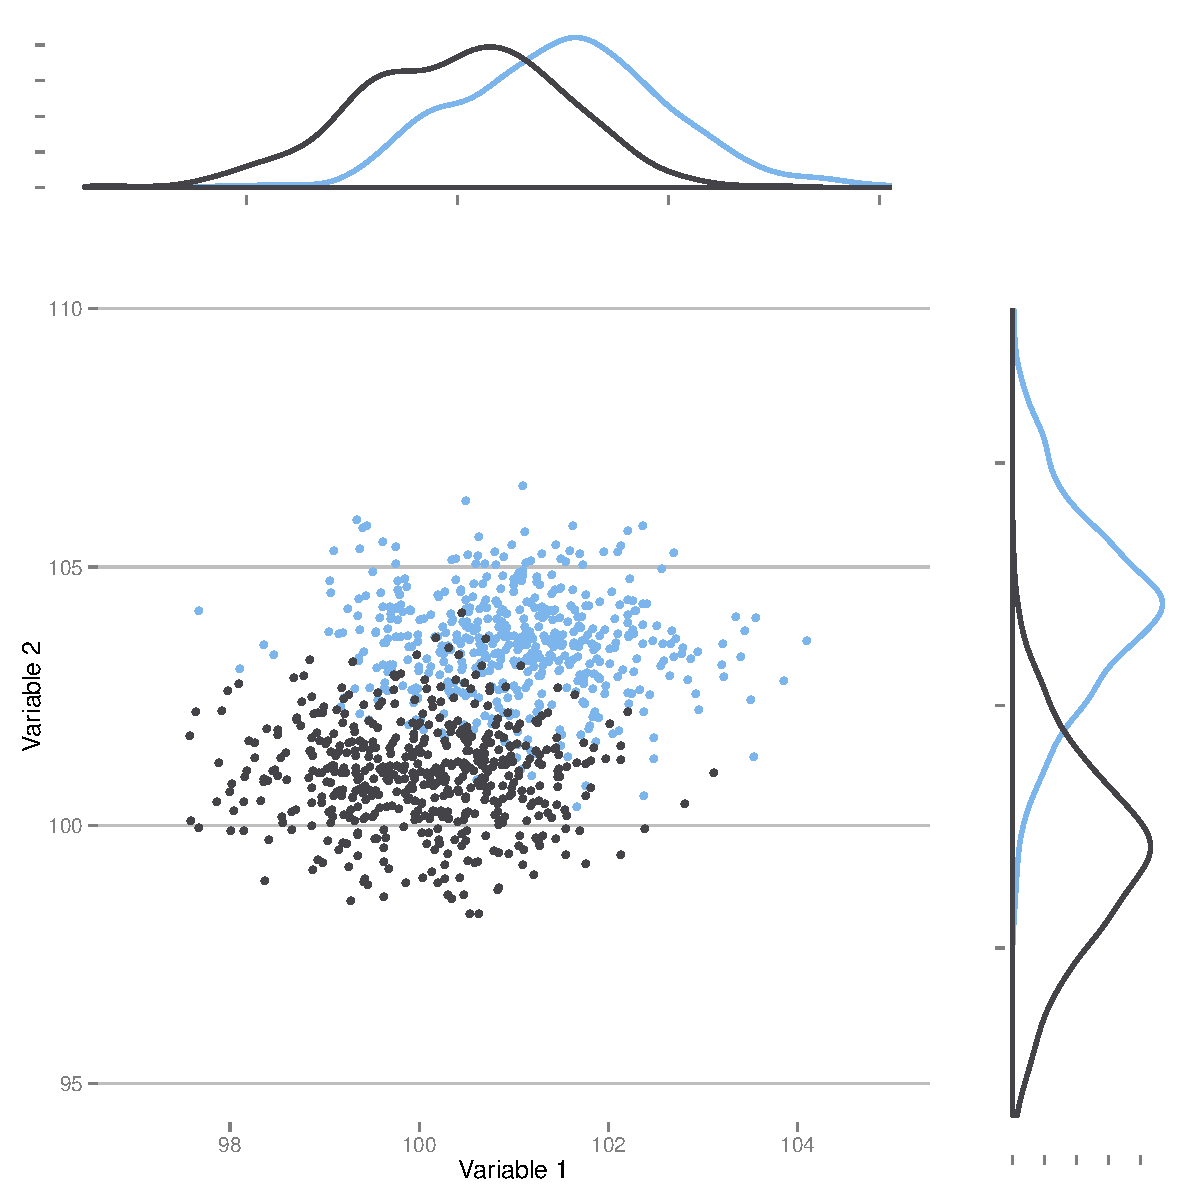
\includegraphics[scale=0.6]{figure/equifinality-variable-effect.pdf}
\caption{Simple example of the effect of variable choice in distinguishing models.  The variable on the X axis displays quite a bit of overlap between models, while the variable on the Y axis distinguishes the models with fairly high accuracy.}
\label{img:variables-equifinality-example}
\end{figure}

\begin{figure}[ht]
\centering
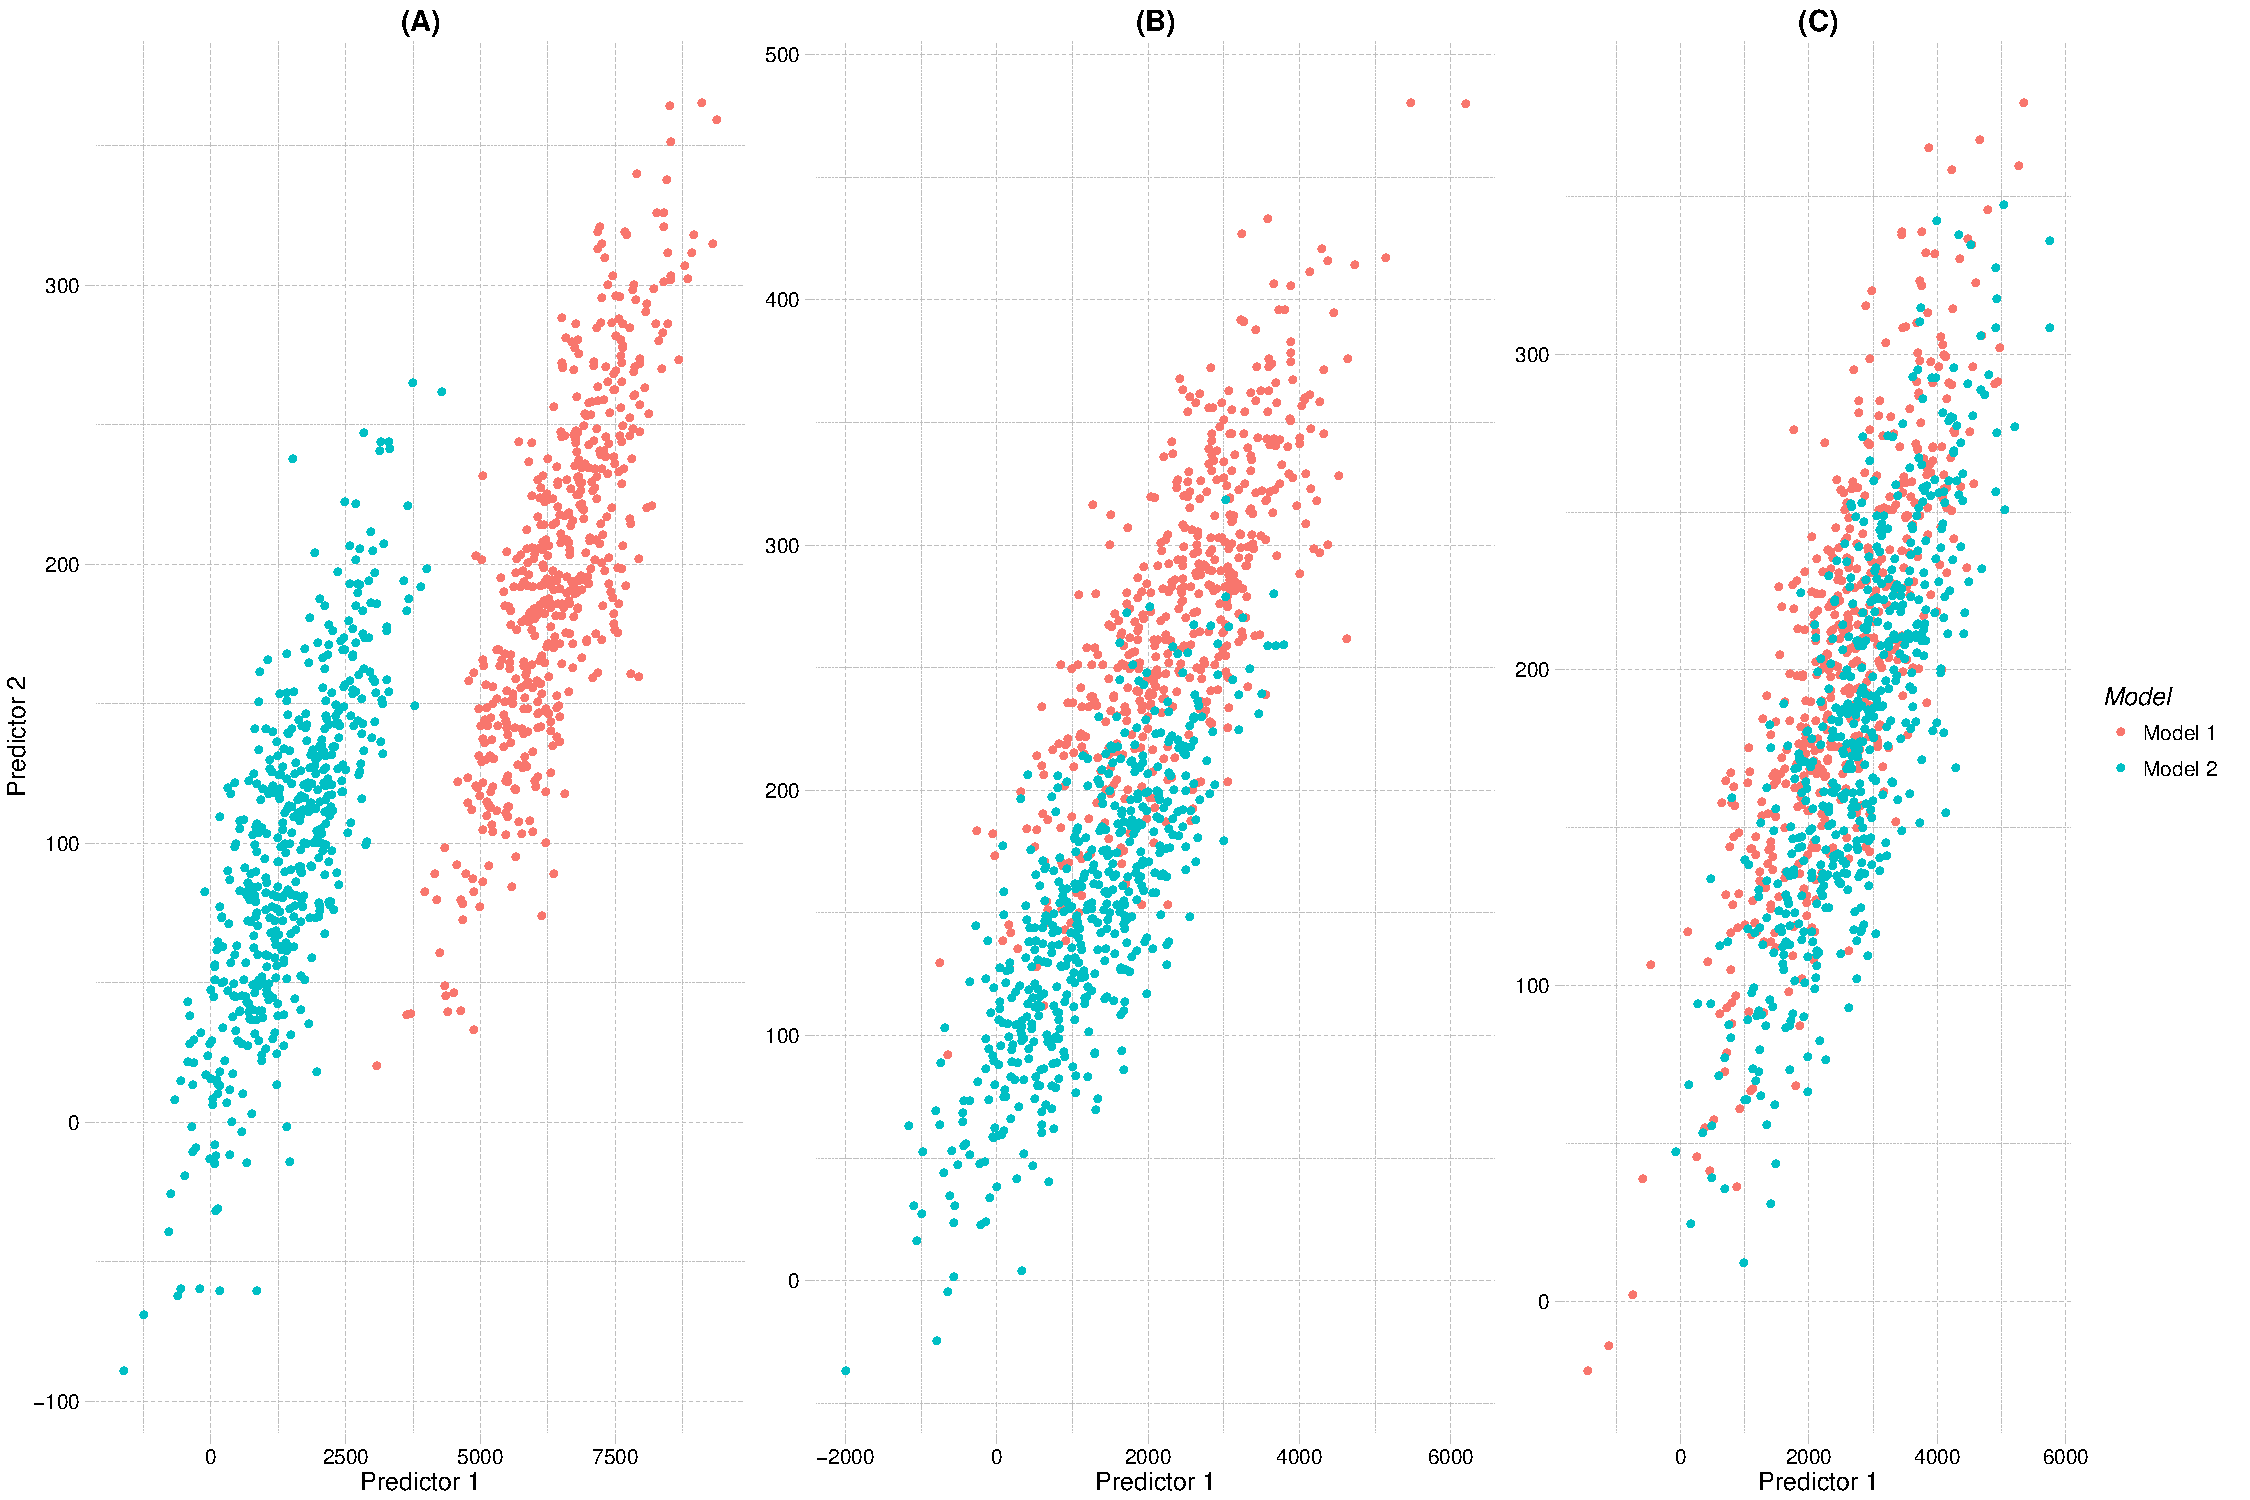
\includegraphics[scale=0.6]{figure/distributional-overlap.pdf}
\caption{Simple example of model outcomes with different degrees of distinguishability: (A) simulated data point from two fully separate models, (B) two models with a limited overlap region, (C) and two models whose outcomes are highly overlapping.}
\label{img:separability-example}
\end{figure}

\begin{figure}[ht]
\centering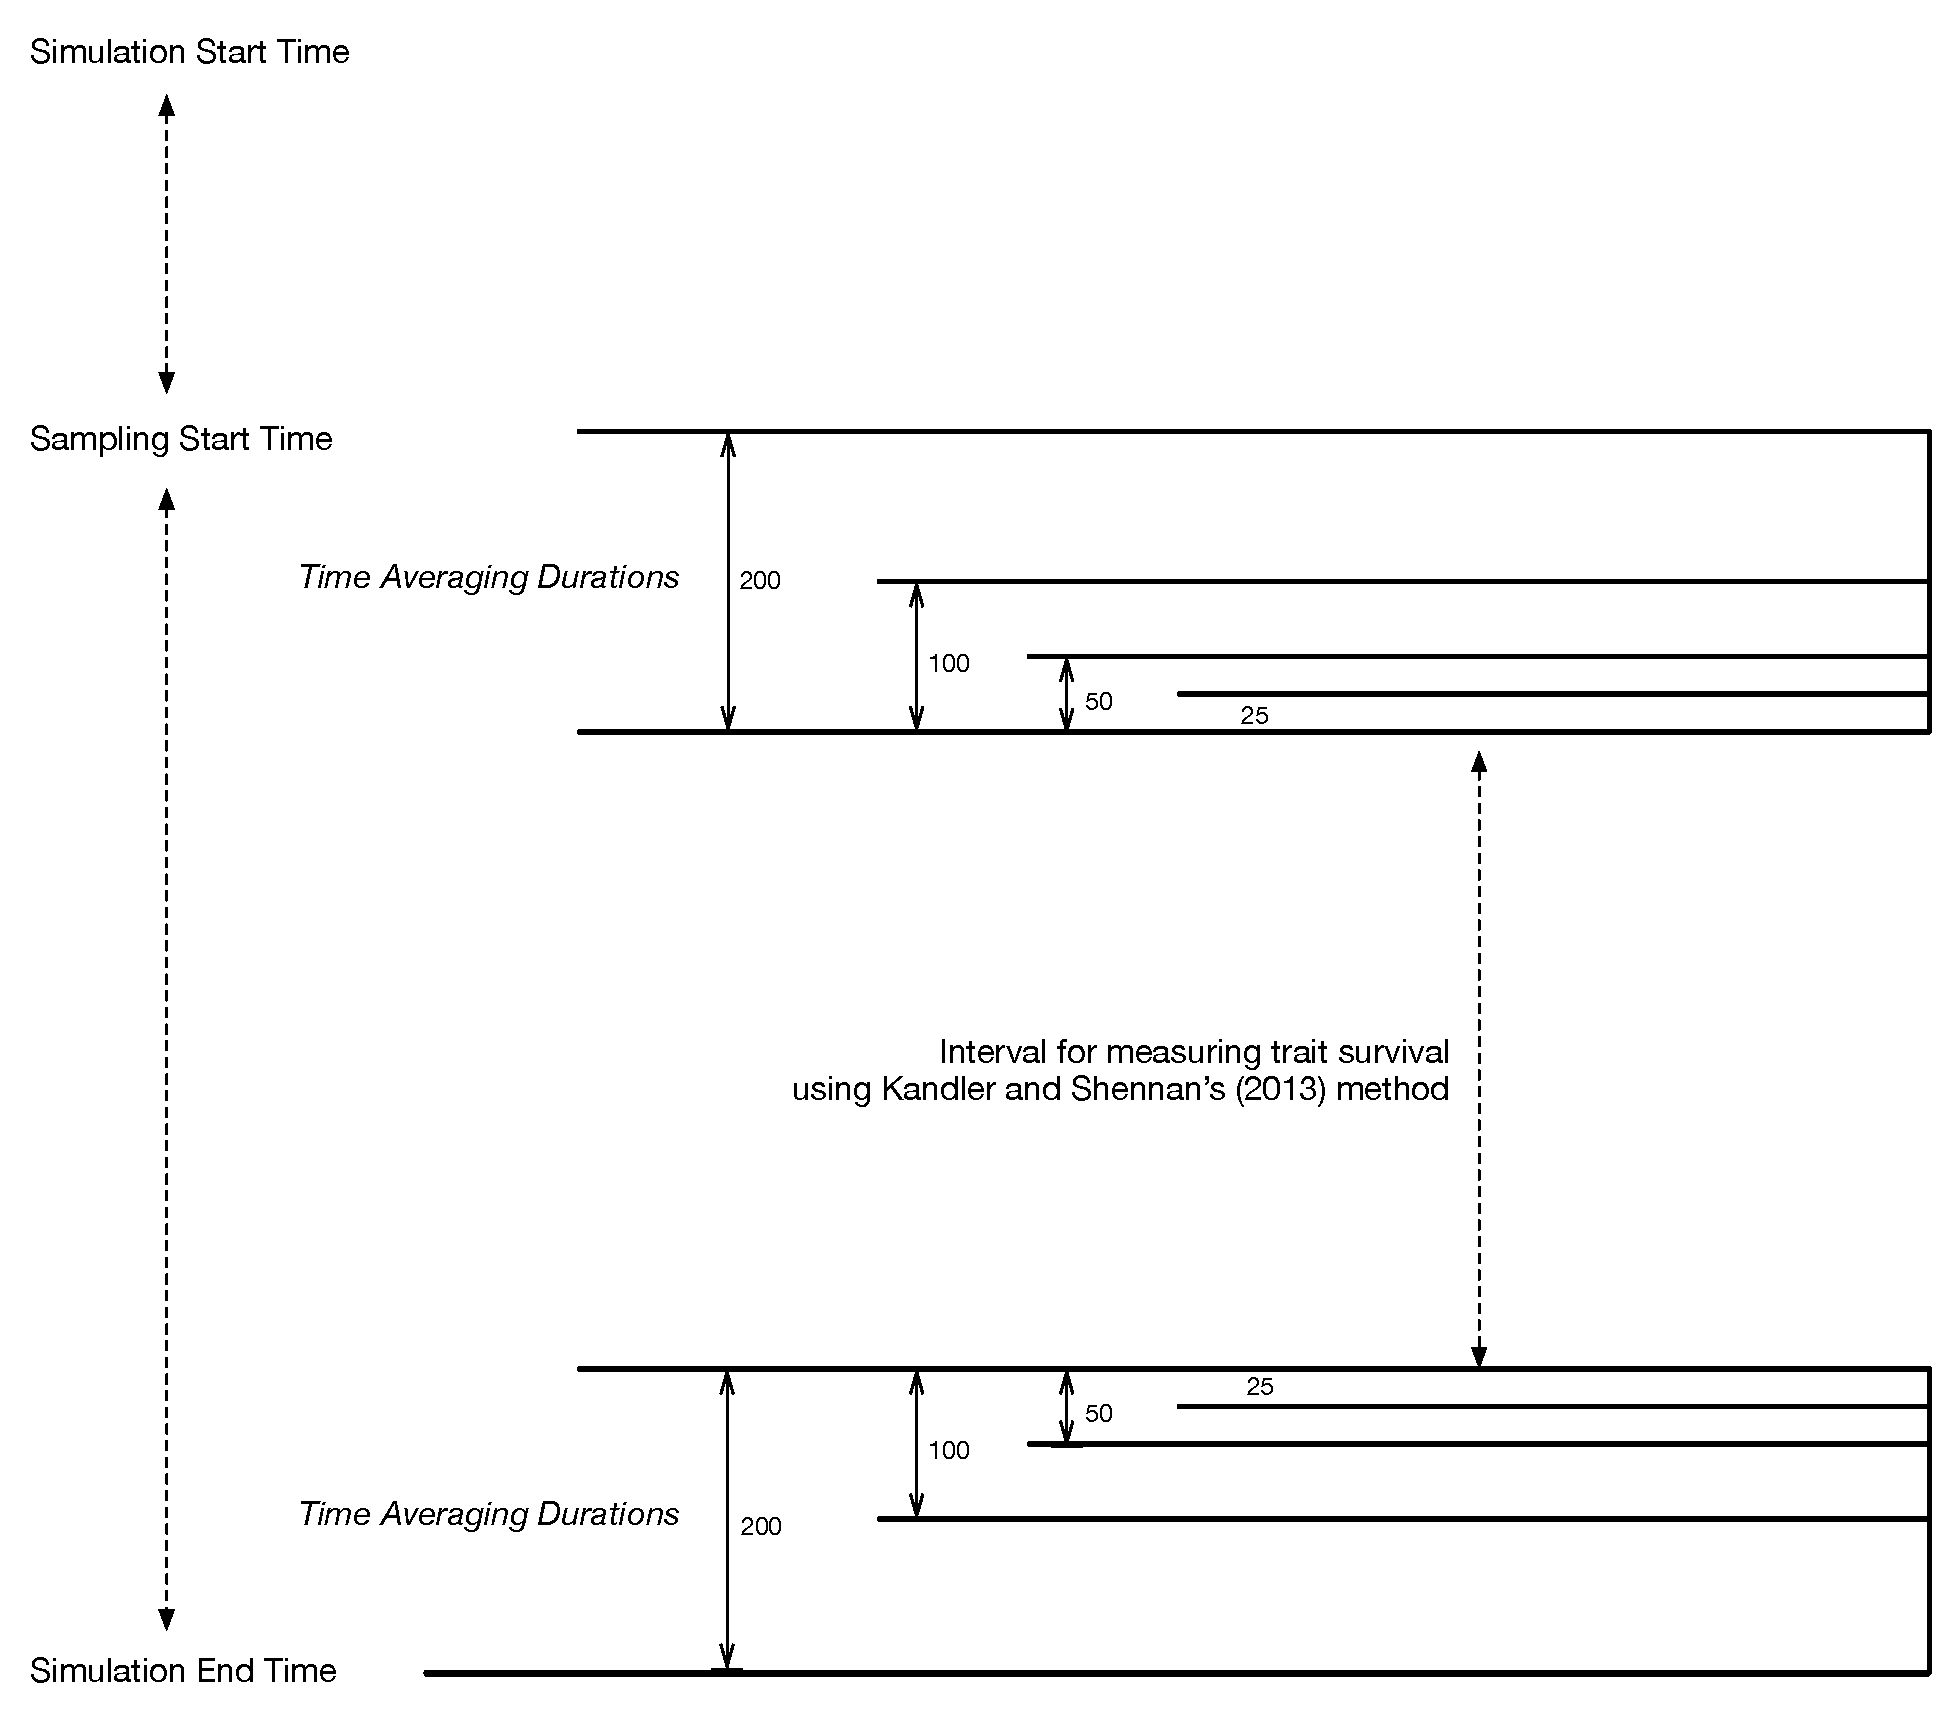
\includegraphics[scale=0.4]{figure/time-averaging-with-kandler-sampling.pdf}
\caption{Schematic of how sampling is implemented in this study.  Time runs from the start of the simulation run at the top, to the end at the bottom.  The interval of time over which we calculate the Kandler-Shennan trait survival is given as a simulation parameter, and represents the gap in the middle of the diagram.  Before and after that gap are windows of successive duration, representing aggregation over 10, 25, 50, and 100 ``generations'' of the simulation.}
\label{img:timeaveraging}	
\end{figure}


\begin{figure}[ht]
\centering
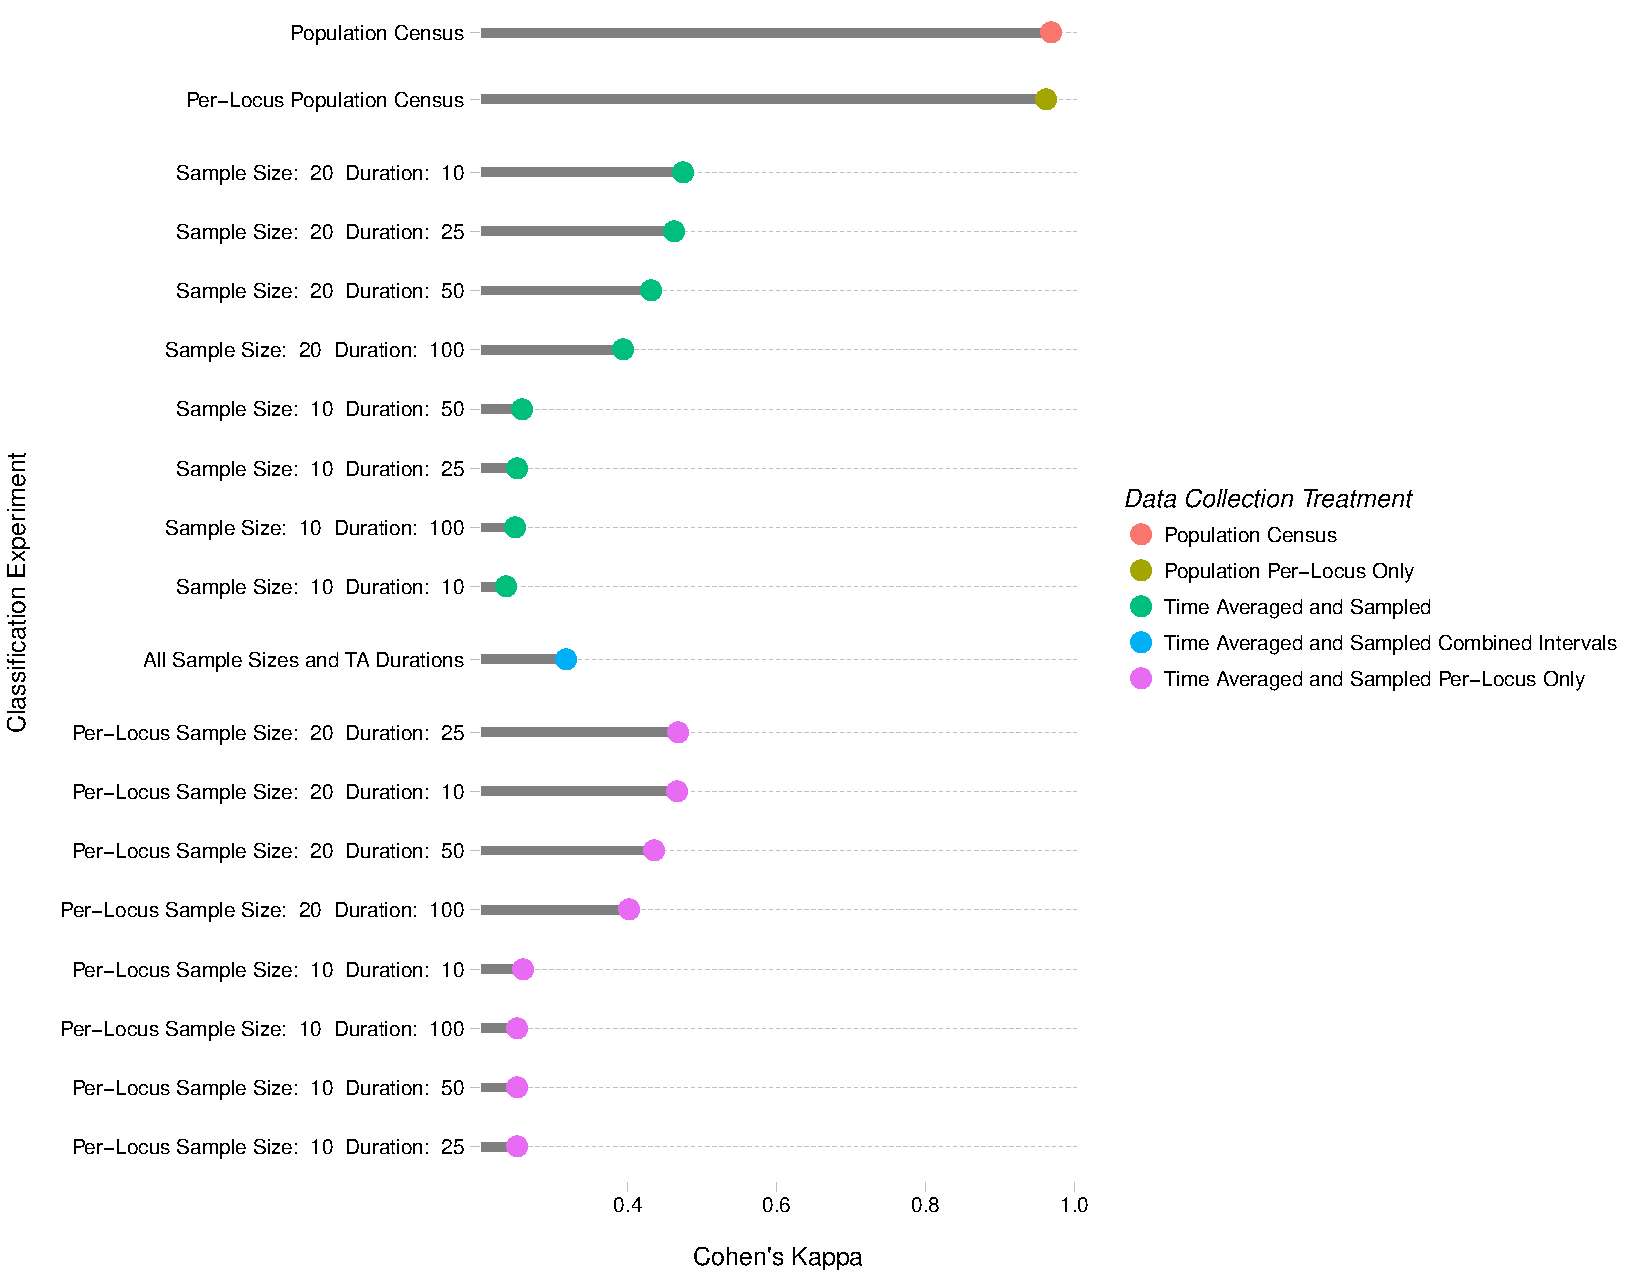
\includegraphics[scale=0.5]{figure/unbiased-biased-kappa-dotchart.pdf}
\caption{Cohen's kappa for correctly predicting whether simulated data points originate from unbiased copying or any of 3 other biased transmission models.  High values of kappa correspond to high accuracy in correctly distinguishing between transmission models, while values well below 0.5 indicate great difficult and low classifier accuracy.  Each line in the dotchart represents a different data collection treatment, and overall the results indicate that significant equifinality exists except when time averaging is absent and a population census (or near equivalent) is available.}
\label{img:unbiased-biased-kappa}
\end{figure}

\begin{figure}[ht]
\centering
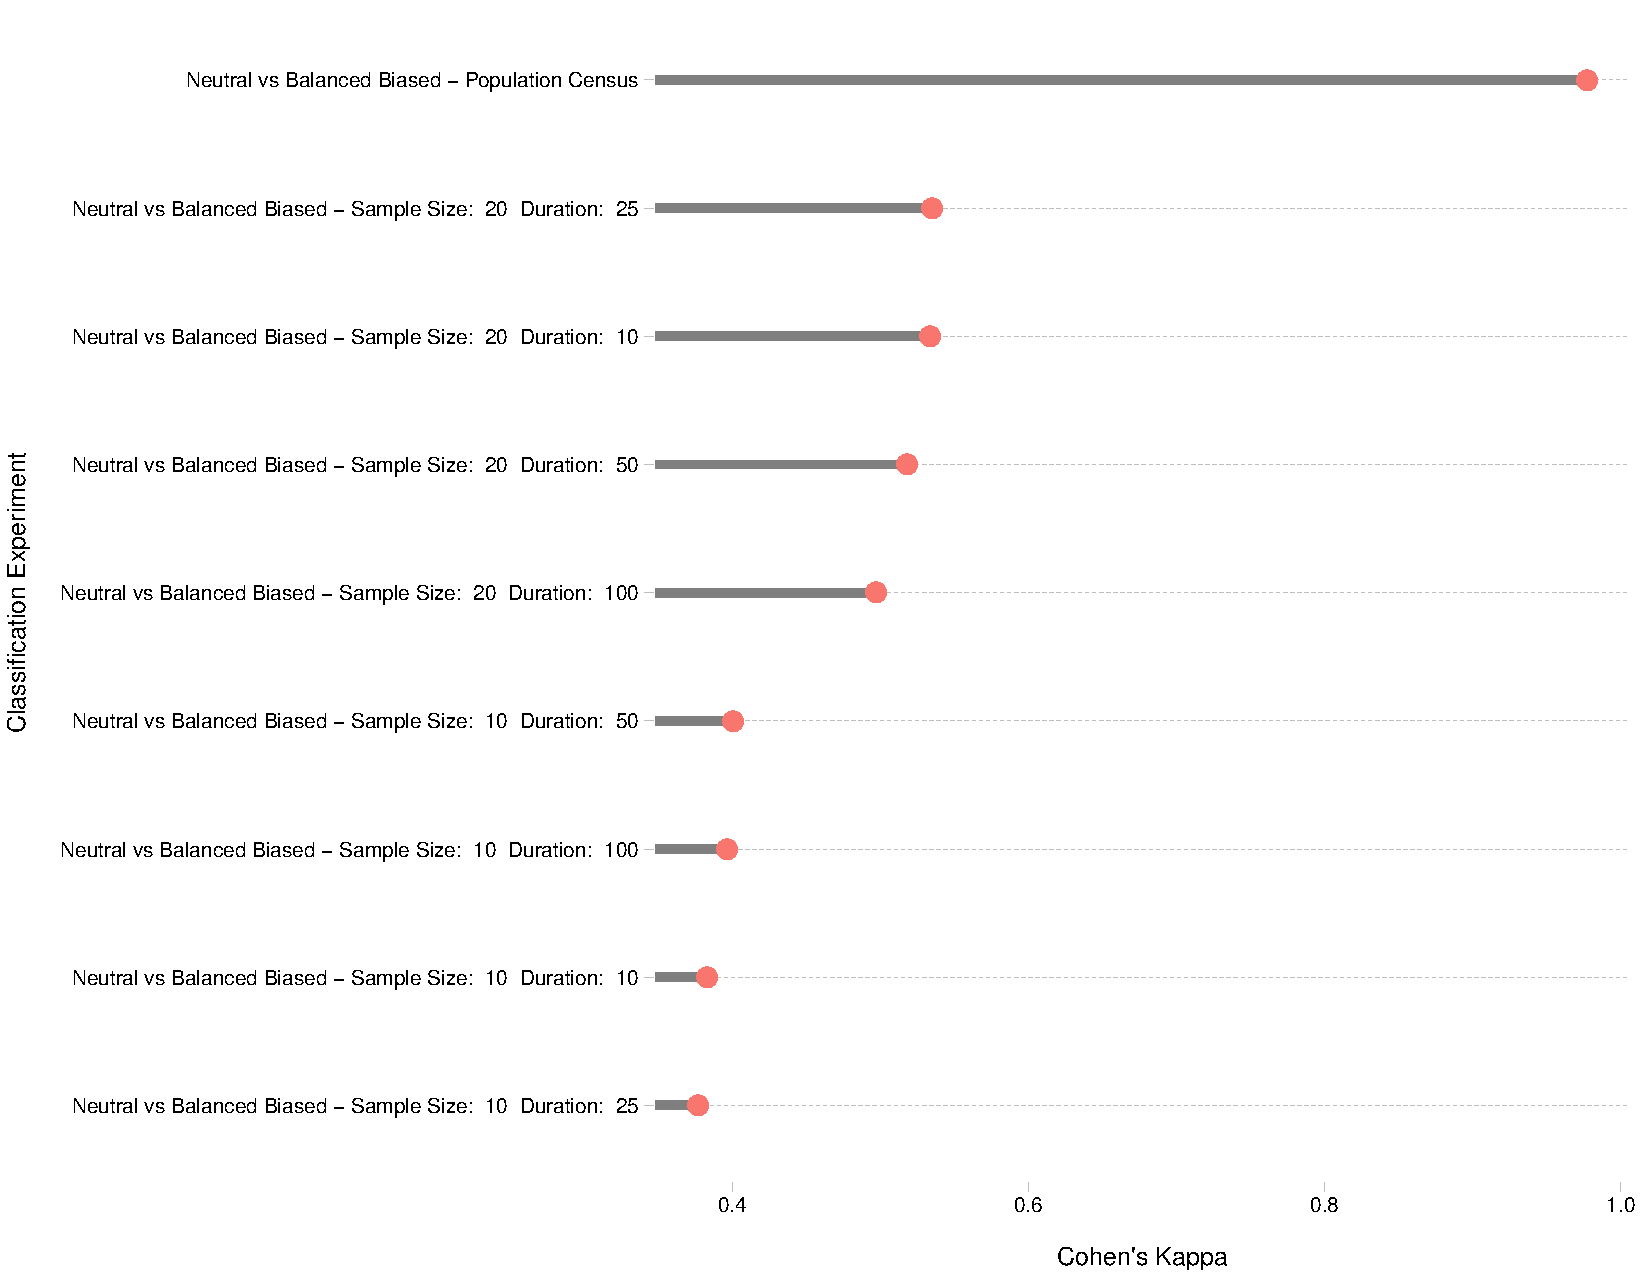
\includegraphics[scale=0.5]{figure/unbiased-balbiased-kappa-dotchart.pdf}
\caption{Cohen's kappa for correctly predicting whether simulated data points originate from unbiased copying or a balanced mixture of pro- and anti-conformist individuals.  Each line in the dotchart represents a different data collection treatment, and overall the results indicate that significant equifinality exists except when time averaging is absent and a population census (or near equivalent) is available.}
\label{img:unbiased-biased-kappa}
\end{figure}

\begin{figure}[ht]
\centering
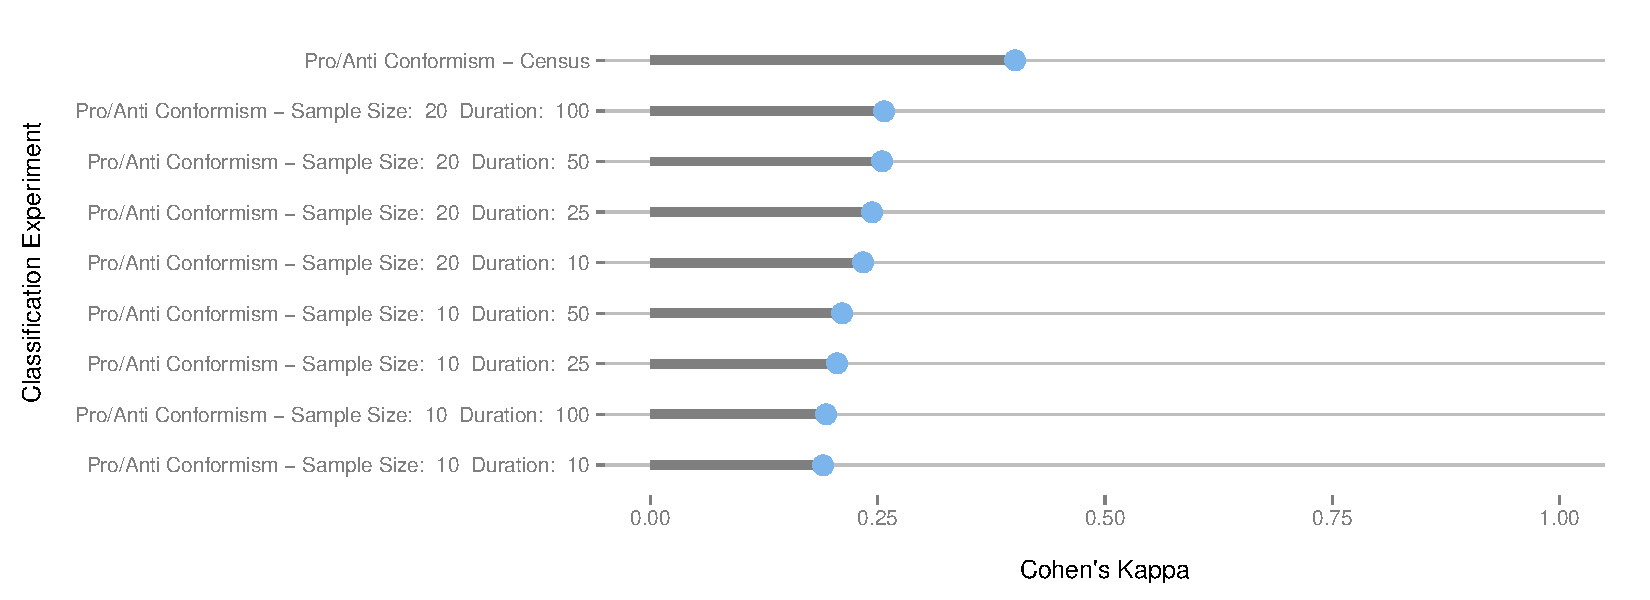
\includegraphics[scale=0.5]{figure/proanticomparison-kappa-dotchart.pdf}
\caption{Cohen's kappa for correctly predicting whether simulated data points originate from a conformist-dominated mixed population versus a mixed population dominated by anti-conformists.  Each line in the dotchart represents a different data collection treatment, and overall the results indicate that strong equifinality exists regardless of the data collection treatment.}
\label{img:proanti-kappa}
\end{figure}

\end{document}

